%---------------------------------------------------------------------------------
%                西南交通大学研究生学位论文:第三章内容
%---------------------------------------------------------------------------------
\chapter{TCP/NC协议实现}
本章主要讲TCP/NC的具体实现,在lossy信道下测试TCP/NC的性能,并与标准的TCP-vegas进行分析对比。
\section{数据包编码}
在阐述数据包编码之前,先简单介绍近世代数的相关概念。
\subsection{有限域与扩域}
\begin{myDef}[阿贝尔群]
	对于一个非空元素集合$G$以及定义在$G$上的一种运算“$*$”( 这里的$*$泛指一种代数运算,如$+$,$-$,$\times$,$\div$,模$m$加$\oplus$,模$m$乘$\odot$等)。若满足以下四个条件:
	\begin{enumerate}[fullwidth,itemindent=2em,label=(\arabic*)]
		\item 封闭性,即$\forall a,b \in G$,$\exists\left(a*b\right)=c\in G$。
		\item 结合性,即$\forall a,b \in G$,$\exists a*\left(b*c\right)=\left(a*b\right)*c$。
		\item 存在唯一一个单位元$e$,即$\forall a \in G$,$\exists a*e=e*a=a$。
		\item $G$中的每个元素各自存在唯一的逆元,即$\forall a \in G$,$\exists {a^{ - 1}} \in G$,使得$a*{a^{-1}}={a^{-1}}*a=e$。这里${a^{-1}}$泛指逆元。
		\item $\forall a,b \in G$,$\exists a*b=b*a$
	\end{enumerate}
	\par
	则称这样的代数系统为阿贝尔群,记做$\left(G,*\right)$\textsuperscript{\cite{zzc2003}}。
\end{myDef}
\begin{myDef}[有限域]
	非空集合$F$含有有限个元素,其中定义了加和乘两种运算,且满足
	\begin{enumerate}[fullwidth,itemindent=2em,label=(\arabic*)]
		\item $F$关于加法构成阿贝尔群,加法恒等元记为0
		\item $F$中所有非零元素对乘法构成阿贝尔群,乘法恒等元记为1
		\item $F$加法和乘法满足分配律
	\end{enumerate}
	\par
	则$F$与这两种运算构成有限域\textsuperscript{\cite{zzc2003}}。
\end{myDef}
\begin{table}[htbp]
	\centering
	\caption{本原多项式$P\left(x\right)=x^{4}+x+1$的根生成的循环群}
	\begin{tabularx}{250pt}{c|c|c}
		\toprule
		\textbf{各次幂$\alpha_{k}$} & \textbf{$\alpha$的多项式}&\textbf{多项式系数$m$重}\\
		\midrule
		$\alpha^{0}$ & 1 &$\left(0001\right)$\\
		\hline
		$\alpha^{1}$ & $\alpha$ &$\left(0010\right)$\\
		\hline
		$\alpha^{2}$ & $\alpha^{2}$ & $\left(0100\right)$\\
		\hline
		$\alpha^{3}$ & $\alpha^{3}$ & $\left(1000\right)$\\
		\hline
		$\alpha^{4}$ & $\alpha+1$ & $\left(0011\right)$\\
		\hline
		$\alpha^{5}$ & $\alpha^{2}+\alpha$ & $\left(0110\right)$\\
		\hline
		$\alpha^{6}$ & $\alpha^{3}+\alpha^{2}$ & $\left(1100\right)$\\
		\hline
		$\alpha^{7}$ & $\alpha^{3}+\alpha+1$ & $\left(1011\right)$\\
		\hline
		$\alpha^{8}$ & $\alpha^{2}+1$ & $\left(0101\right)$\\
		\hline
		$\alpha^{9}$ & $\alpha^{3}+\alpha$ & $\left(1010\right)$\\
		\hline
		$\alpha^{10}$ & $\alpha^{2}+\alpha+1$ & $\left(0111\right)$\\
		\hline
		$\alpha^{11}$ & $\alpha^{3}+\alpha^{2}+\alpha$ & $\left(1110\right)$\\
		\hline
		$\alpha^{12}$ & $\alpha^{3}+\alpha^{2}+\alpha+1$ & $\left(1111\right)$\\
		\hline
		$\alpha^{13}$ & $\alpha^{3}+\alpha^{2}+1$ & $\left(1101\right)$\\
		\hline
		$\alpha^{14}$ & $\alpha^{3}+1$ & $\left(1001\right)$\\
		\hline
	\end{tabularx}
	\label{SHUYU}
\end{table}
\par
有限域提供了一个有限集,在该有限集上明确地定义且有效地实现了加法、减法、乘法及除法运算( 减法可以转换为加法,除法可以转换为乘法),并允许系统使用矩阵、行列式、高斯消元等线性代数中常见的运算工具来解决该域上的联立线性方程组问题。
\par
我们在讲到$GF\left(q\right)$时,经常顺带会讲到$GF\left(q^{m}\right)$,表示$GF\left(q\right)$的扩域。扩域里至少存在一个本原元$\alpha$,它的各次幂$\alpha^{0}$,$\alpha^{1}$,$\alpha^{2}$,$\dots$,$\alpha^{q^{m}-2}$构成了扩域$GF\left(q^{m}\right)$的全部非零域元素。表\ref{SHUYU}展示的就是以本原多项式$P\left(x\right)=x^{4}+x+1$对应的本原元的各次幂生成的$GF\left(2^4\right)$的全部非零元素。
\subsection{数据包的运算}
由于从TCP层下来的数据包都是字节流,如何抽象出我们在第\ref{xianxingbianma}小节中谈到的报文概念呢?进一步地,我们如何对这些报文进行各种操作,如加减乘除呢?
\par
将数据包分解成字节,先对字节进行加减乘除的操作,拼接得到的结果是可行的。这解决了以何种角度刻画数据包的问题。对于数据包的运算,如果是在实数域上进行各种代数运算,则会涉及到进位的问题,不好处理。例如,$p_{1}$和$p_{2}$这两个数据包的二进制形式为$p_{1}=\left(1010\ 1010\right)$和$p_{2}=\left(1111\ 0000\right)$。在实数域上计算得到$p_{3}=p_{1}+p_{2}$,则$p_{3}=\left(1\ 1001\ 1010\right)$,$p_{1}$和$p_{2}$都是8个比特,但是$p_{3}$却是$9$比特,出现了进位,导致我们的处理很麻烦。
\par
上一小节中提到的有限域和扩域是解决数据包运算问题的关键。有限域是一种代数结构,也存在着和实数域中一样的加减乘除等运算,并且各个元素进行加减乘除得到的结果也在有限域中。具体实现过程如下:
\begin{enumerate}[fullwidth,itemindent=2em,label=(\arabic*)]
	\item 确定有限域的大小。由于在计算机中按字节操作最方便,一个字节8个比特,刚好可以看做是一个8位向量。因此,选定扩域$GF\left(2^8\right)$。
	\item 选定一个在$GF\left(2^8\right)$下的生成元$\alpha$,$\alpha$的各次幂和零元素一起构成整个扩域,即$GF\left(2^8\right)=\{0,1,\alpha,\alpha^2,\alpha^3,\dots,\alpha^{254}\}$。$GF\left(2^8\right)$可用的生成元如表格\ref{GENERATOR}。这里我们选定$\alpha=0x03$作为生成元。换句话说,$\forall e \in GF\left(2^8\right) $,且$e \neq 0$,$e=\left(0x03\right)^{k}\left(k=0,1,2,\dots,254\right)$。
	\item 构建以$0x03$作为生成元的$Exponential$表,$Exp\_tab[256]$和$Logarithm$表,$Log\_tab[256]$。其中$Exp\_tab[i]=\left(0x03\right)^{i}$,$\left(0x03\right)^{Log\_tab[i]}=i$。所有代数运算都在$GF\left(2^8\right)$下进行。$Exp\_tab[256]$和$Log\_tab[256]$如表\ref{Exptab}和表\ref{Logtab}。如此,我们在有限域上的运算仅仅通过查表就可以得到。例如,通过表$Log\_tab[256]$可以查到$\left(0x03\right)^{0x01}=0x03$,$\left(0x03\right)^{0xc6}=0x07$,那么$0x03*0x07=\left(0x03\right)^{0x01}*\left(0x03\right)^{0xc6}=\left(0x03\right)^{0x01+0xc6}=0x9$。通过查表法,可以快速的实现$GF\left(2^8\right)$上的乘除运算。
\end{enumerate}
\begin{table}[htbp]
	\caption{$GF\left(2^8\right)$可用的生成元( 十六进制 )}
	\centering
\begin{tabular}{cccccccccccccccc}
	%%\rowcolor[gray]{.8}
	\toprule
 03 & 05&06& 09 &0b& 0e &11& 12 &13 &14& 17& 18 &19 &1a& 1c& 1e \\
 1f &21 &22 &23& 27 &28& 2a &2c &30 &31 &3c &3e& 3f &41& 45& 46 \\
 47& 48& 49& 4b& 4c& 4e& 4f& 52& 54& 56 &57 &58& 59& 5a& 5b& 5f \\
 64 &65& 68& 69& 6d& 6e& 70 &71 &76& 77& 79 &7a &7b& 7e &81 &84 \\
 86& 87 &88& 8a& 8e& 8f& 90& 93 &95& 96 &98& 99& 9b &9d &a0 &a4 \\
 a5& a6& a7 &a9& aa &ac &ad &b2& b4& b7& b8& b9 &ba &be &bf &c0 \\
 c1 &c4& c8& c9& ce &cf& d0& d6 &d7& da& dc &dd& de& e2 &e3& e5 \\
 e6& e7& e9& ea& eb& ee &f0& f1& f4& f5& f6& f8& fb& fd & fe &ff \\
	\bottomrule
\end{tabular}
	\label{GENERATOR}
\end{table}


\begin{table}[htb]
	\caption{Log\_tab[256]}
	\centering
	\begin{tabular}{cccccccccccccccc}
		%%\rowcolor[gray]{.8}
		\toprule
 0&0&19&1&32&2&1a&c6&4b&c7&1b&68&33&ee&df&3\\
64&4&e0&e&34&8d&81&ef&4c&71&8&c8&f8&69&1c&c1\\
7d&c2&1d&b5&f9&b9&27&6a&4d&e4&a6&72&9a&c9&9&78\\
65&2f&8a&5&21&f&e1&24&12&f0&82&45&35&93&da&8e\\
96&8f&db&bd&36&d0&ce&94&13&5c&d2&f1&40&46&83&38\\
66&dd&fd&30&bf&6&8b&62&b3&25&e2&98&22&88&91&10\\
7e&6e&48&c3&a3&b6&1e&42&3a&6b&28&54&fa&85&3d&ba\\
2b&79&a&15&9b&9f&5e&ca&4e&d4&ac&e5&f3&73&a7&57\\
af&58&a8&50&f4&ea&d6&74&4f&ae&e9&d5&e7&e6&ad&e8\\
2c&d7&75&7a&eb&16&b&f5&59&cb&5f&b0&9c&a9&51&a0\\
7f&c&f6&6f&17&c4&49&ec&d8&43&1f&2d&a4&76&7b&b7\\
cc&bb&3e&5a&fb&60&b1&86&3b&52&a1&6c&aa&55&29&9d\\
97&b2&87&90&61&be&dc&fc&bc&95&cf&cd&37&3f&5b&d1\\
53&39&84&3c&41&a2&6d&47&14&2a&9e&5d&56&f2&d3&ab\\
44&11&92&d9&23&20&2e&89&b4&7c&b8&26&77&99&e3&a5\\
67&4a&ed&de&c5&31&fe&18&d&63&8c&80&c0&f7&70&7\\
		\bottomrule
	\end{tabular}
	\label{Logtab}
\end{table}


\begin{table}[htb]
	\caption{Exp\_tab[256]}
	\centering
	\begin{tabular}{cccccccccccccccc}
		%%\rowcolor[gray]{.8}
		\toprule
 1& 3& 5& f&11&33&55&ff&1a&2e&72&96&a1&f8&13&35\\
5f&e1&38&48&d8&73&95&a4&f7& 2& 6& a&1e&22&66&aa\\
e5&34&5c&e4&37&59&eb&26&6a&be&d9&70&90&ab&e6&31\\
53&f5& 4& c&14&3c&44&cc&4f&d1&68&b8&d3&6e&b2&cd\\
4c&d4&67&a9&e0&3b&4d&d7&62&a6&f1& 8&18&28&78&88\\
83&9e&b9&d0&6b&bd&dc&7f&81&98&b3&ce&49&db&76&9a\\
b5&c4&57&f9&10&30&50&f0& b&1d&27&69&bb&d6&61&a3\\
fe&19&2b&7d&87&92&ad&ec&2f&71&93&ae&e9&20&60&a0\\
fb&16&3a&4e&d2&6d&b7&c2&5d&e7&32&56&fa&15&3f&41\\
c3&5e&e2&3d&47&c9&40&c0&5b&ed&2c&74&9c&bf&da&75\\
9f&ba&d5&64&ac&ef&2a&7e&82&9d&bc&df&7a&8e&89&80\\
9b&b6&c1&58&e8&23&65&af&ea&25&6f&b1&c8&43&c5&54\\
fc&1f&21&63&a5&f4& 7& 9&1b&2d&77&99&b0&cb&46&ca\\
45&cf&4a&de&79&8b&86&91&a8&e3&3e&42&c6&51&f3& e\\
12&36&5a&ee&29&7b&8d&8c&8f&8a&85&94&a7&f2& d&17\\
39&4b&dd&7c&84&97&a2&fd&1c&24&6c&b4&c7&52&f6& 1\\
		\bottomrule
	\end{tabular}
	\label{Exptab}
\end{table}
乘法和除法的关键代码见代码\ref{GCAL},\emph{gmul}实现乘法,\emph{gdiv}实现除法。
	\begin{lstlisting}[caption=gmul和gdiv实现,label={GCAL},language={[ANSI]C}]
	unsigned char gmul (unsigned char a, unsigned char b)
	{
	return Exp_tab[Log_tab[a] ^ Log_tab[b]];
	}
	unsigned char gdiv (unsigned char a, unsigned char b)
	{
	return Exp_tab[Log_tab[a] ^ Log_tab[b]];
	}
	\end{lstlisting}

\par
我们以两\ref{GCAL}个数据包$p_{1}$和$p_{2}$的运算为例,说明如何对数据包进行编码。假定数据包$p_{1}$和$p_{2}$都为一个2字节的报文,以比特流的形式表示,$p_{1}=\{1010\ 0101\ 0110\ 1111\}$,$p_{2}=\{1111\ 0000\ 1101\ 0110\}$,我们需要计算$p_{encoded}=7p_{1} \oplus 13p_{2}$的值。步骤如下:
\begin{enumerate}[fullwidth,itemindent=2em,label=(\arabic*)]
	\item 取$p_{1}$和$p_{2}$的第一个字节,分别是$\{1010\ 0101\}$和$\{1111\ 0000\}$,对应的十进制为$D_{p_1}=165$和$D_{p_2}=240$。计算$gmul\left(7,D_{p_1}\right)$和$gmul\left(13,D_{p_2}\right)$的值,分别是$0xc6$和$0xc4$。则$p_{encoded}$的第一个字节为$0xc4 \oplus 0xc6=0x02$,二进制表示为$\{0000\ 0010\}$。
	\item 同样的方法处理$p_{1}$和$p_{2}$的第二个字节,结果为$\{1010\ 0111\}$。
	\item 拼接两个结果得到$p_{encoded}=\{0000\ 0010\ 1010\ 0111\}$。
\end{enumerate}
\section{技术方案}
\subsection{开发平台}
TCP/NC的实现需要参与到协议栈的流程中去,涉及到内核开发。因此,只能选择开源的Linux平台。考虑到TCP/NC的应用场景主要是无线网络环境中的移动终端,本文决定选择一款嵌入式设备,在其上部署实现TCP/NC协议,以验证分析其在真实环境中的性能。
\par
Raspberry Pi是一款基于Linux的单板机电脑,由英国的树莓派基金会开发。基于ARM架构的Raspberry Pi使用博通( Broadcom )公司的BCM28XX系列处理器,主频从700MHz到1.2GHz不等\textsuperscript{\cite{rasp}}。不仅如此,Raspberry Pi还引出了40个管脚,便于我们使用KGDB调试工具调试内核。图\ref{RASP_EPS}即为本文选择的Raspberry Pi 二代B型,主频900MHz,板载Ethernet网口,4个USB接口及HDMI视频输出。
\begin{figure}[htbp]
	\centering
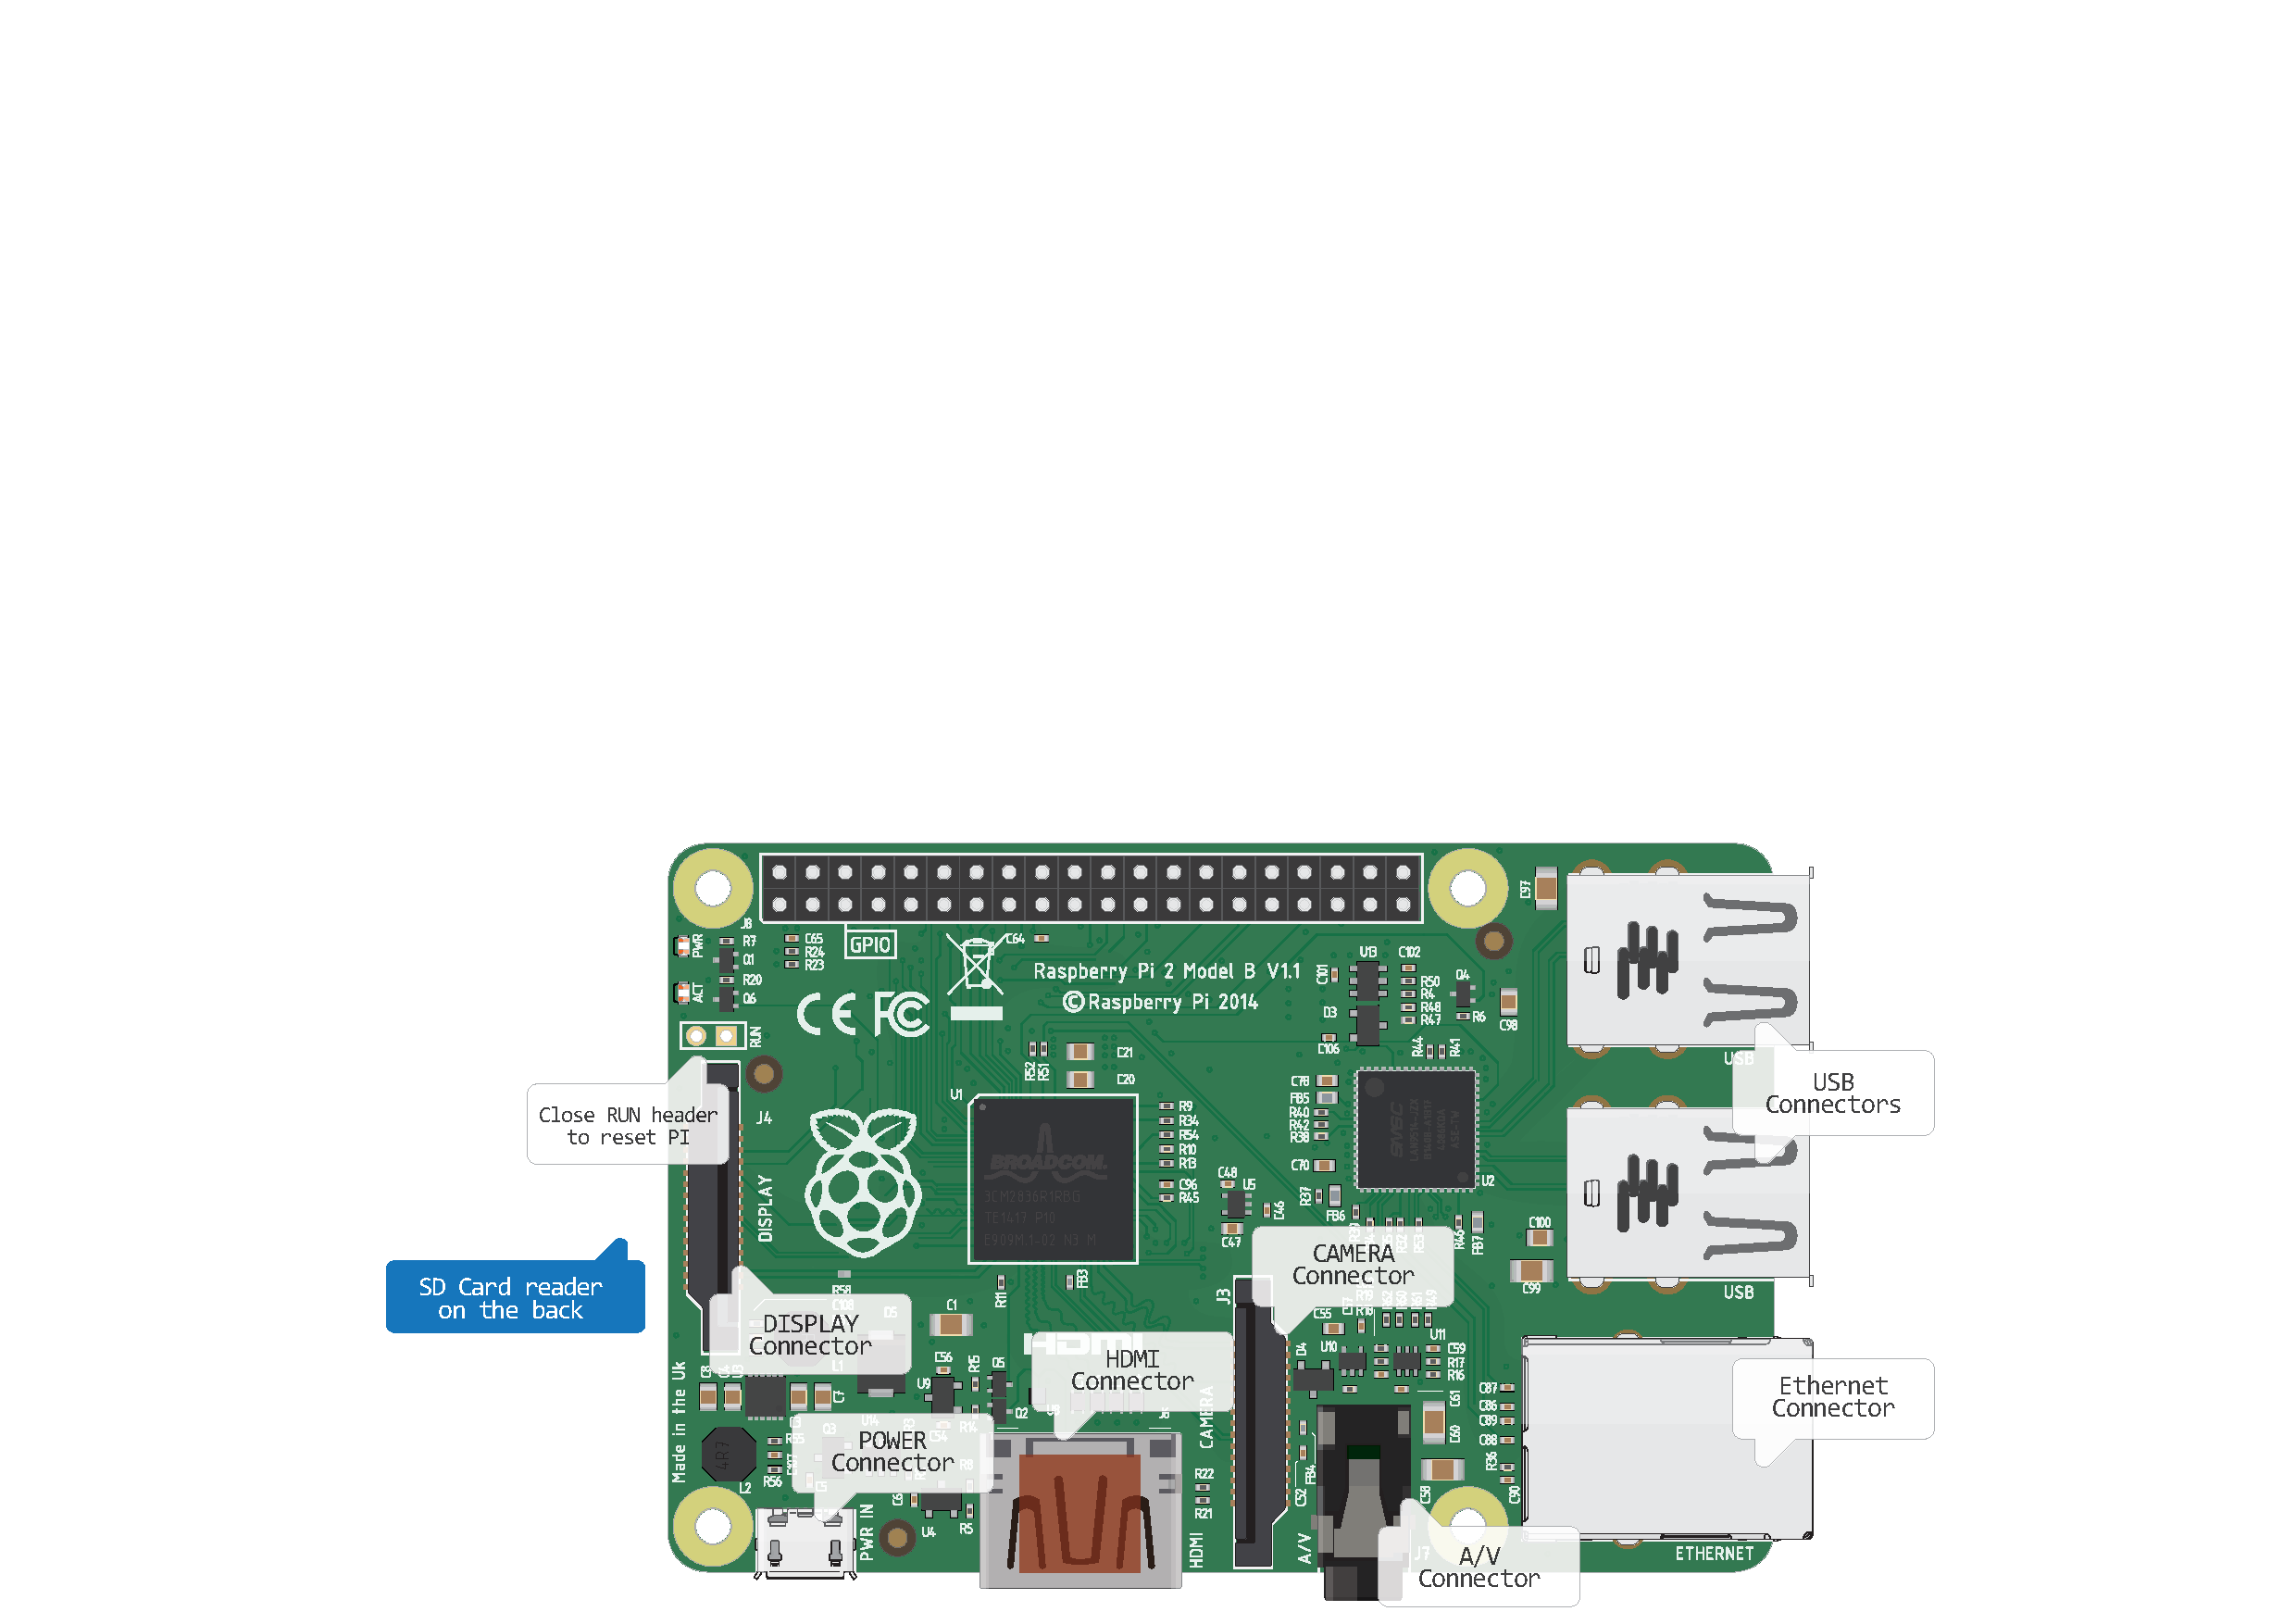
\includegraphics[width=6in]{figures/rasp.pdf}
\caption{Raspberry Pi二代B型}
\label{RASP_EPS}
\end{figure}
系统选择上,本文选择使用树莓派基金会的Debian系统,Linux内核版本为3.18\footnote{内核源码下载地址:\url{https://github.com/raspberrypi/linux}}。内核调试方案则选择使用KGDB调试工具,支持内核源码级别调试。
\subsection{Netfilter}
NC层实施方案有两种。第一种是直接在内核的TCP协议源码上更改,添加我们的NC层各个模块,然后再编译内核源码;第二种则是利用Linux内核提供给用户用于处理网络封包的框架——Netfilter,很多防火墙软件都是基于Netfilter开发的。考虑到工程复杂度,本文选择的是Netfilter框架。
\begin{figure}[htbp]
	\centering
	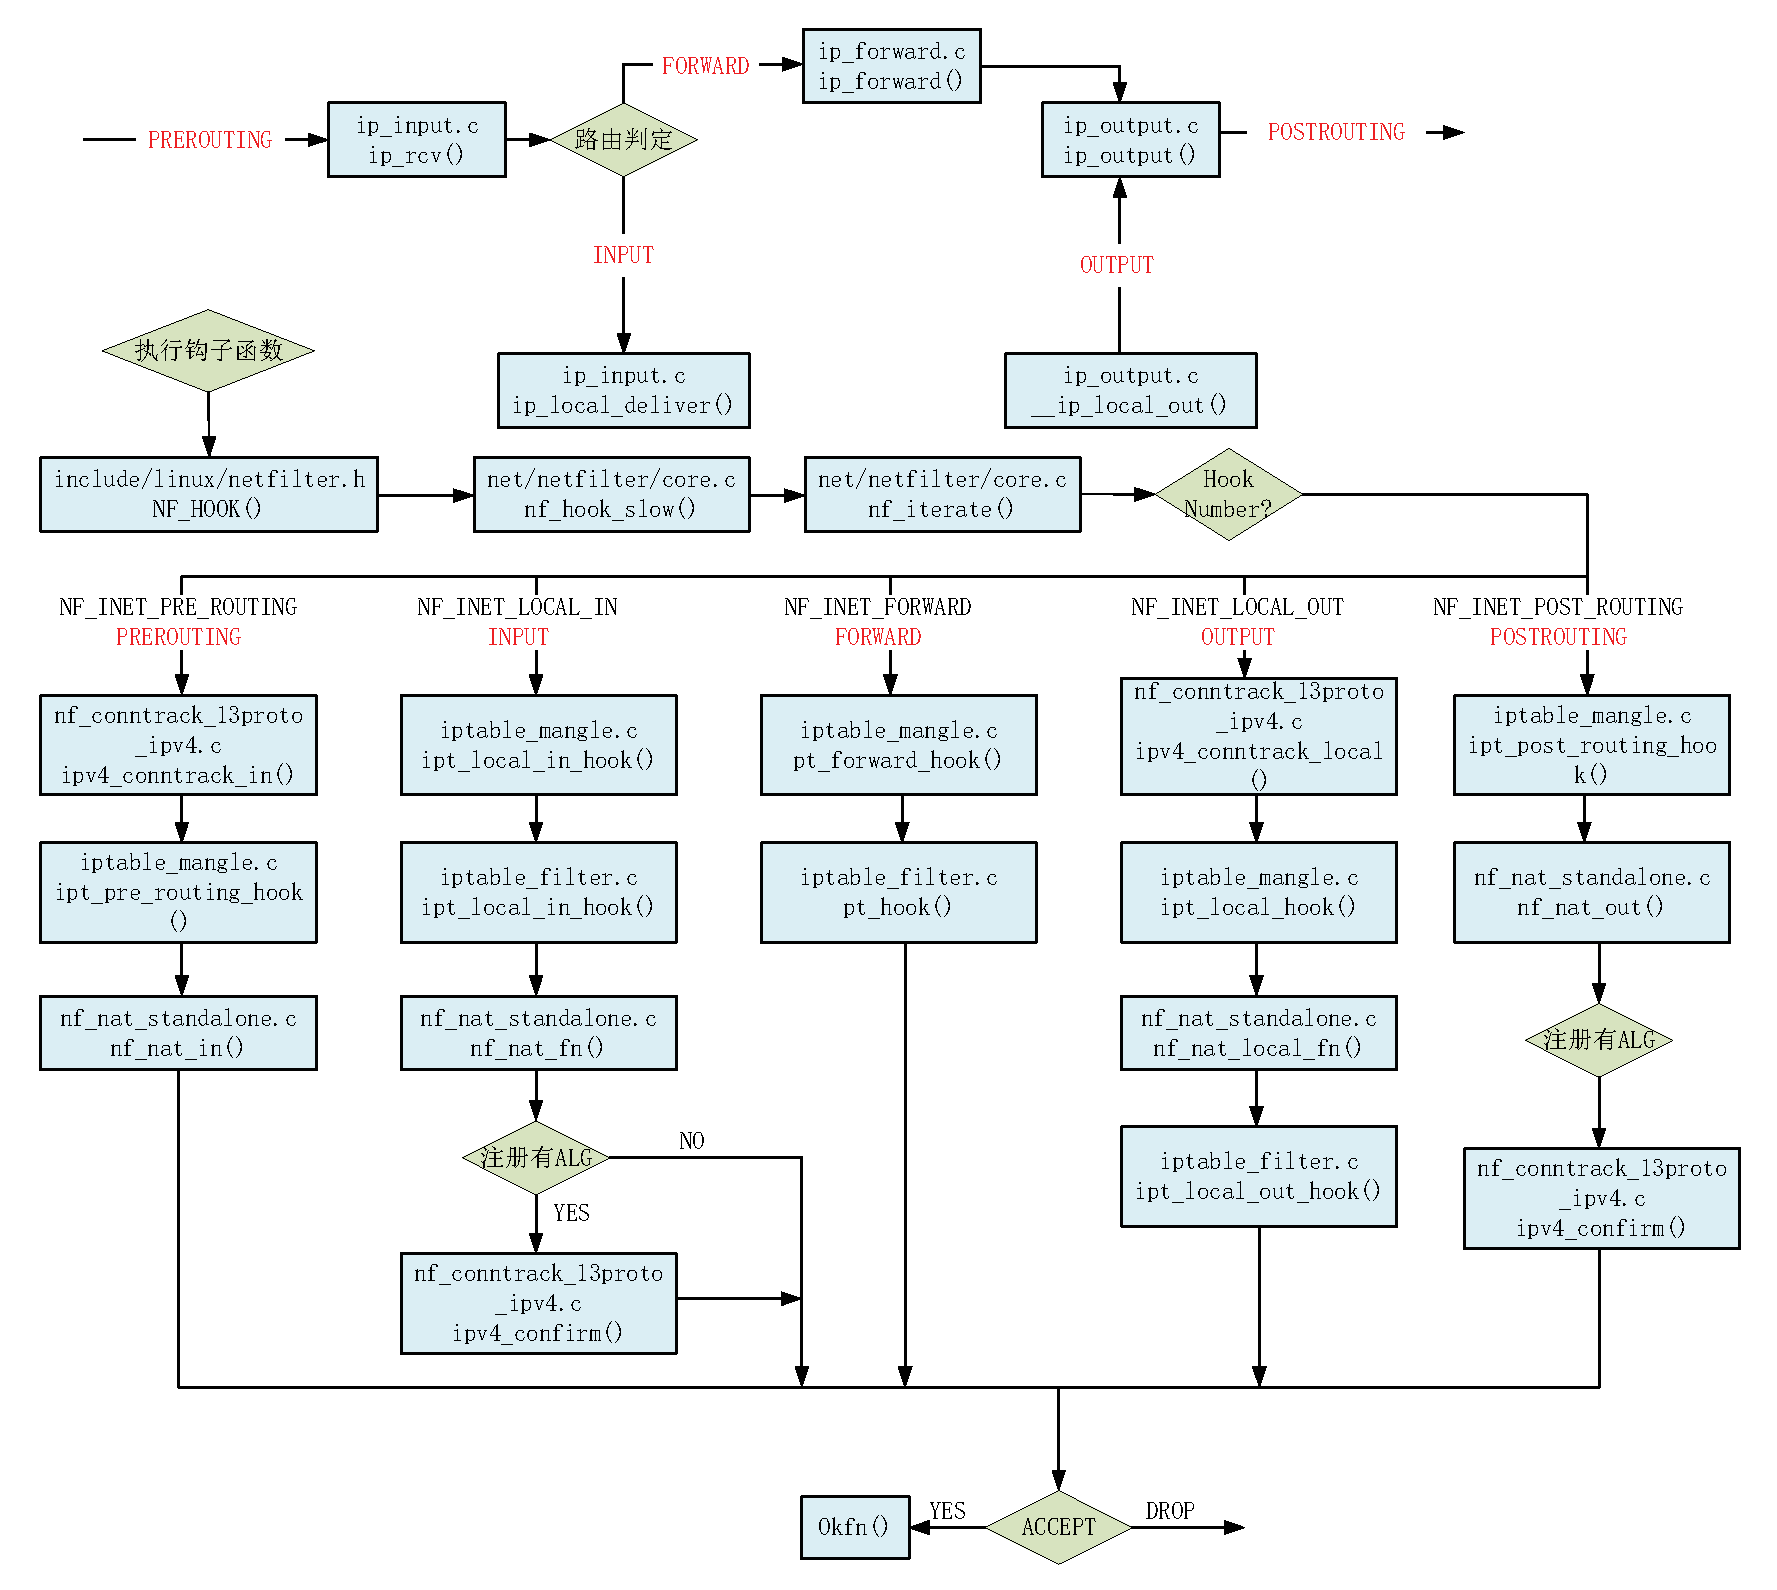
\includegraphics[width=6in]{figures/packetflow.eps}
	\caption{Netfilter框架及其在内核源码中调用关系}
	\label{NETFILTER_EPS}
\end{figure}
Linux中最常用、最基本的防火墙软件称为$iptables$。$iptables$防火墙通过与Linux内核网络协议栈的包过滤钩子交互来工作。这些内核钩子被称为Netfilter框架。Linux系统中允许注册钩子程序的点有5个。数据包在路过Linux的网络协议栈时( 出去或者进来 ) 将触发这些钩子,允许注册这些钩子的函数处理处在钩子点处的报文。数据包所触发的钩子取决于数据包是传入还是传出,数据包的目的地,以及数据包在上一个钩子点是否被丢弃或拒绝。
\par
以下钩子表示网络协议栈中有标准定义的钩子点:
\begin{itemize}[leftmargin=.5in]
	\item \textbf{NF\_IP\_PRE\_ROUTING}:数据包在进入协议栈之后,在对这个数据包作出路由决定之前,会触发这个钩子。
	\item \textbf{NF\_IP\_LOCAL\_IN}:如果一个数据包是送往本机的,那么在作出这个路由决定之后,就会触发这个钩子。
	\item \textbf{NF\_IP\_FORWARD}:如果一个数据包经过路由判定是送往其他机器的,那么就会触发这个钩子。
	\item \textbf{NF\_IP\_POST\_ROUTING}:在数据包离开本机之前,会触发这个钩子。触发这个钩子的数据包包括从本机发往网络的包和仅仅是经过本机的路由判定后发往网络中其他机器的报文。
	\item \textbf{NF\_IP\_LOCAL\_OUT}:数据包由本地发出去时,会执行挂载在这个钩子上的模块。
\end{itemize}
\par
图\ref{NETFILTER_EPS}展示的是Netfilter的框架及其在内核源码的调用关系。想要在这些钩子点注册的内核模块还需要提供一个优先级,用于决定在触发这个钩子时,按照一个什么顺序执行挂载在这些钩子上的模块。Netfilter中的钩子函数有固定的返回值,常用的有如下几个:
\begin{itemize}[leftmargin=.5in]
	\item NF\_ACCEPT:当前钩子函数对数据包的处理结束,通知hook chain继续遍历其他的钩子函数。
	\item NF\_DROP:终止hook chain执行,并释放当前的skb。
	\item NF\_STOLEN:同样终止hook chain执行,但告诉Netfilter由我这个hook来接管skb的生命周期。
\end{itemize}
本论文的NC层就是架构于Netfilter框架,将我们的NC层编解码模块$ncout$和$ncin$分别挂在NF\_IP\_LOCAL\_OUT和NF\_IP\_LOCAL\_IN这两个钩子点上。凡是从TCP层下来的报文都会进入编码模块,凡是从IP层上来的报文都会进入解码模块。这样我们的NC层就接管了进出本机的报文,达到了将NC层插入TCP层和IP层之间的目的。
\subsection{报文获取}
NC层在NF\_IP\_LOCAL\_IN和NF\_IP\_LOCAL\_OUT这两个钩子点获得的都是单独的报文,其形式为\emph{sk\_buff}结构体。\emph{sk\_buff}可能是Linux网络代码中最重要的数据结构,包含了数据包所需的所有控制信息,代表已接收或正要传输的数据的报头\textsuperscript{\cite{linux网络技术内幕}}。在内核中,\emph{sk\_buff}被组织成链表,这样就可以快速地将\emph{sk\_buff}从一个链表移动到另一个链表。数据包在Linux的网络协议栈的不同层之间传递,其体现形式就是不同层的函数对一个数据包对应的\emph{sk\_buff}进行各种操作。如\emph{sk\_buff}结构体中的data指针,其指向当前协议层的有效数据内容的起始地址。对于传输层,有效数据包括用户数据和传输层协议头部;对于网络层,有效数据包括用户数据、传输层协议和网络层协议头部;对于数据链路层,有效数据包括用户数据、传输层协议头部、网络层协议头部和链路层协议头部。因此,不同协议层需要移动\emph{sk\_buff}的data指针,以添加首部。这比在不同层之间拷贝数据包效率高得多。图\ref{SKBUFFEPS}为\emph{sk\_buff}数据结构示意图。
\begin{figure}[htbp]
	\centering
	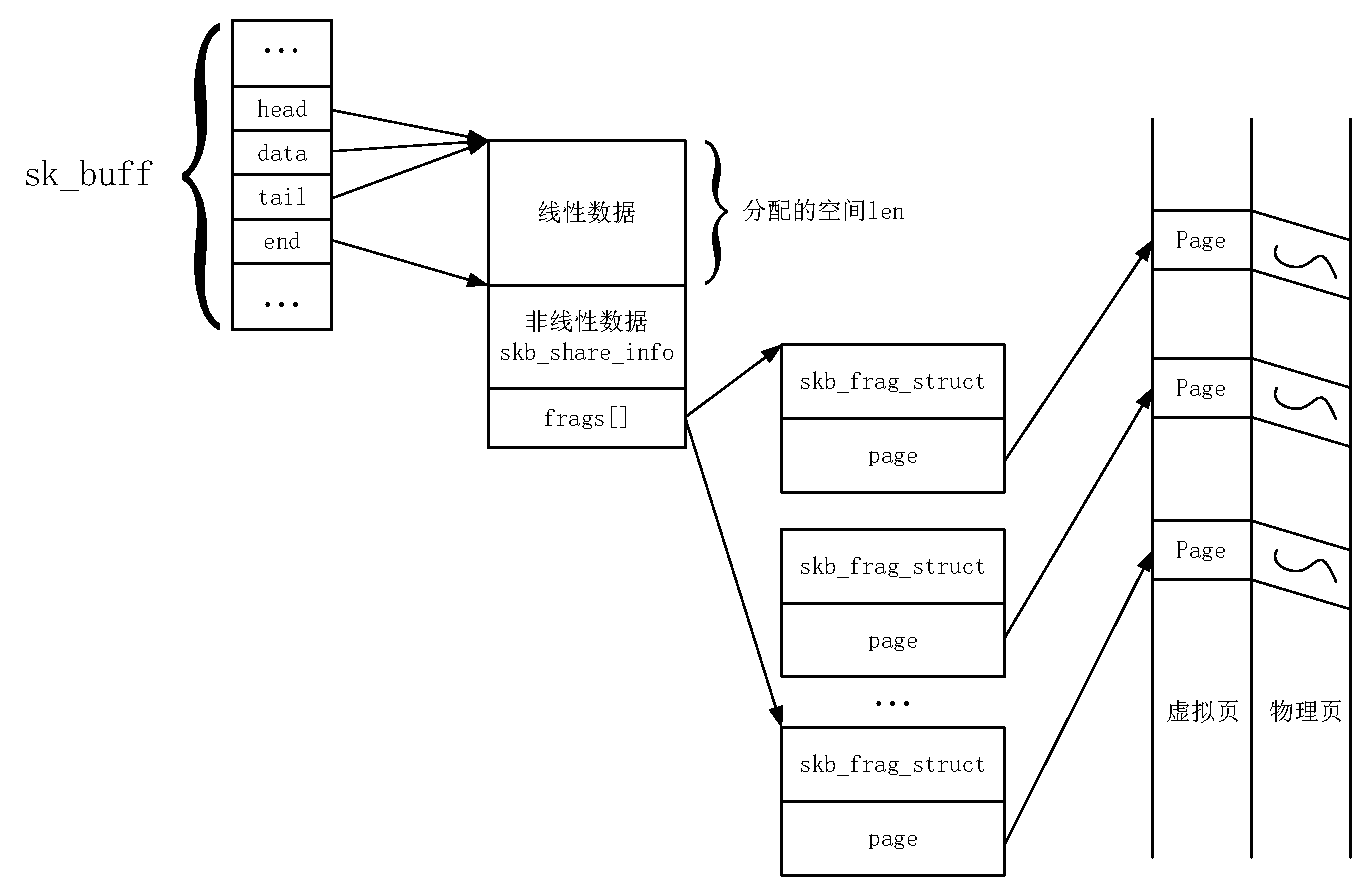
\includegraphics[width=6in]{figures/skbuff.eps}
	\caption{skbuff结构}
	\label{SKBUFFEPS}
\end{figure}

\par

上一小节讲到,Netfilter框架为NC层的实现提供了方案。每当有数据包从网络中发往本机时,就会调用挂载在NF\_IP\_LOCAL\_IN上的模块( 或者说是函数 );当有数据包从本机发往网络中时,就会调用挂载在NF\_IP\_LOCAL\_OUT上的模块。内核模块则通过\emph{struct sk\_buff *skb}来对数据包进行各种操作。代码\ref{NCOUT}即为挂载在NF\_INET\_LOCAL\_OUT处的\emph{ncout}函数体( 函数实现已省略 ),TCP层下来的报文从此函数处进入NC层,然后被编码发往网络。\emph{ncout}函数是由用户编写,但是其参数类型和个数都是固定不变的。用户通过参数列表中的\emph{struct sk\_buff * skb}来对从TCP层下来的报文做进一步处理。如果数据包从TCP层下来,通过\emph{struct sk\_buff *skb},我们可以获得TCP的头部信息如源端端口、目的端口,也可以获得去掉TCP头部的用户数据;如果数据包从下层下来,我们可以移动data指针获取对方的IP地址及用户数据。网络编码层利用这些信息建立一个维护NC连接的控制块,对数据包进行编码。
	\begin{lstlisting}[caption=NF\_INET\_LOCAL\_OUT钩子点函数,label={NCOUT},language={[ANSI]C}]
	static unsigned int ncout(unsigned int hooknum,struct sk_buff * skb,const struct net_device *in,
	const struct net_device *out,int (*okfn) (struct sk_buff *))
	{
	//NC层处理流程	
	} 
	\end{lstlisting}

\section{NC层关键技术}
\subsection{系统框架}
图\ref{JIAGOU_EPS}展示的是TCP/NC的实现架构,虚线框内的就是NC层。对于从TCP层下来的报文,首先要根据TCP报文头部信息判定是何种报文。如果是控制报文,如TCP连接建立的三次握手、RST报文等,则交由控制报文处理模块进行分类处理。控制报文无需经过编解码即可发往IP层。如果从TCP层下来的是普通报文,数据报文需要被送到编码模块进行编码,编码后的数据包需要添加NC头部,填写NC层的控制信息,如编码包的系数、长度等;纯ACK报文( 不带数据 ),也需要添加NC头部,主要是为了不浪费向对端传递NC层的相关信息的机会。
\par
从IP层上来的报文也需要经过数据包类别判定。非NC层报文,即控制报文,直接交给控制报文处理模块处理,然后交给上层TCP层。NC报文,纯ACK则在提取NC层有用信息后再交付给上层TCP层;数据报文则送到解码模块进行解码。不论解码成功,亦或是仅仅看到某个报文( see a packet ),解码模块都需要和NC层控制单元交互信息,以便让NC层控制单元决定是否向TCP连接的对方回复ACK。
\begin{figure}[htbp]
	\centering
	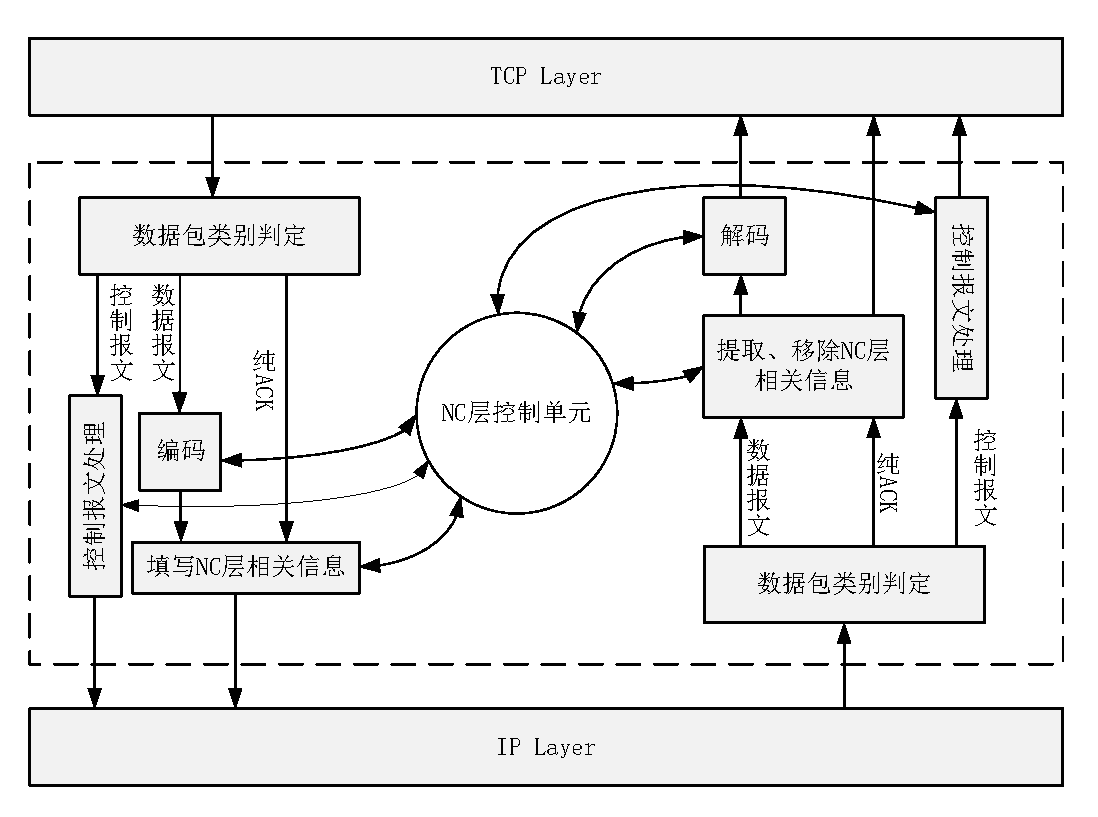
\includegraphics[width=5in]{figures/jiagou.eps}
	\caption{TCP/NC实现架构}
	\label{JIAGOU_EPS}
\end{figure}

\subsection{NC头部设计}
NC层发往下层IP层的报文都需要添加一个NC头部,其中需要填写当前的线性组合报文是由哪几个原始报文组成,及各个原始报文的系数、长度。解码模块利用这些信息才可以进行相关的解码操作,恢复出原始数据包。本文TCP/NC实现中所选的数域是$GF\left(2^8\right)$,因此每个报文的系数都是一个字节大小。
图\ref{CODINGHEADER_EPS}展示的是NC头部的布局。各个字段的含义如下:
\begin{itemize}[leftmargin=.5in]
	\item 源端口和目的端口:这两个端口号和源IP、目的IP一起唯一标识一个NC层的连接。从TCP数据报文的头部可以获得这两个信息。
	\item $Base$: 表示TCP层中还未被确认的数据中第一个字节的序号。这个域可以从\emph{struct tcp\_sock}中的snd\_una域获得。解码端利用这个值来决定哪些报文可以从缓存中删除。
	\item $Start$:参与生成当前编码包的原始报文中序号最靠前的一个原始报文的起始序号。
	\item $Res$:用于分辨NC报文和TCP报文。
	\item $RecvWnd$:对方的接收窗口值,这个接收窗口的值由TCP连接的对方根据它的解码缓存修改得到。
	\item $NCACK$:NC层的确认序号。这个序号值会被交付给上层TCP。
	\item $n$:表示当前这个线性组合报文是由多少个原始报文组成的。
	\item $WS$:扩展因子,其含义与标准TCP中TCP报头的扩展因子一样,用于与$RecvWnd$一起确定接收窗口的值
	\item $len_{i}$:参与生成当前编码包的第$i$个原始报文的长度。
	\item $\alpha_{i}$:参与生成当前编码包的第$i$个原始报文的系数。
\end{itemize}
\begin{figure}[htbp] 
	\centering
	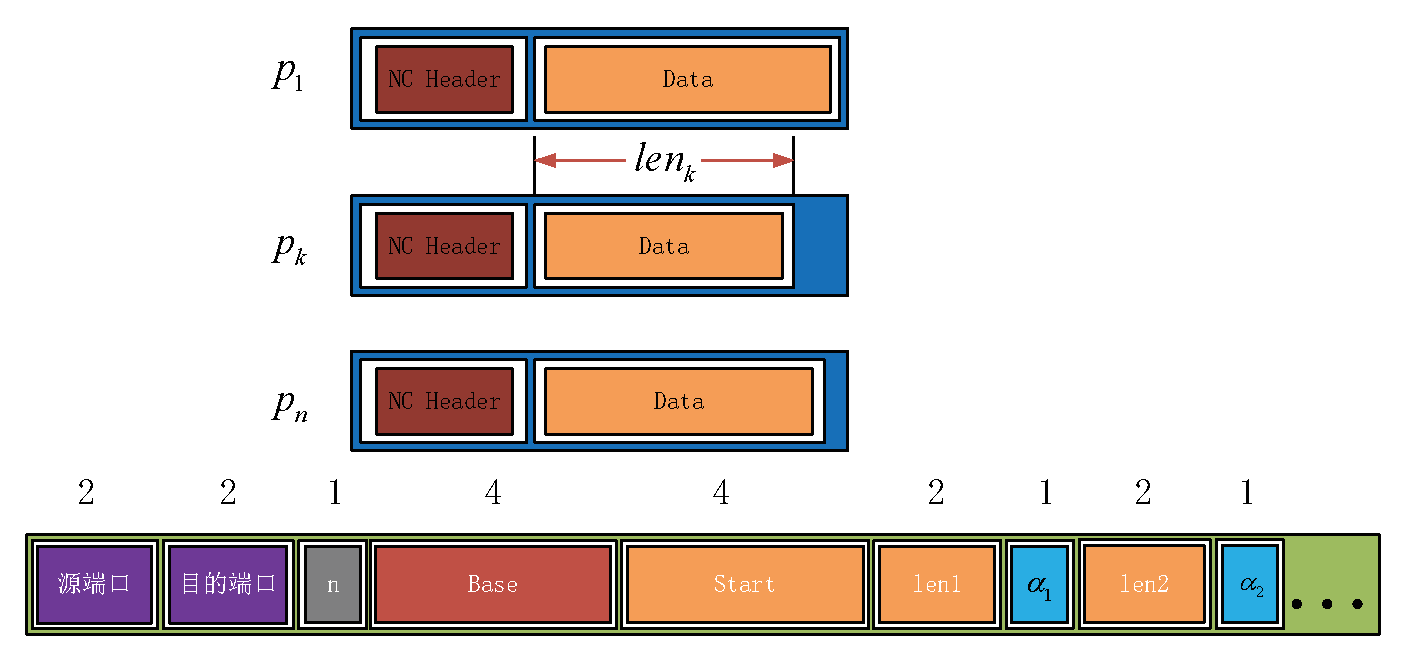
\includegraphics[width=5in]{figures/codingheader.eps}
	\caption{NC层头部}
	\label{CODINGHEADER_EPS}
\end{figure}
\par
\emph{Base}和\emph{Start}都是32比特,和标准TCP头部的\emph{seq}字段长度一致。$len_{i}$则占用2个字节,足够表示一个数据包的长度。以图\ref{CODINGHEADER_EPS}所示布局,一个编码包将需要多耗费$24+3n\left(n \ge 1\right)$个字节。其实还可以将报头开销进一步减小。例如,由于NC头部已经包含了端口信息、扩展因子、ACK序号、接收窗口,可以将它们从TCP的头部去掉,然后解码端在解码出相应报文后,再将相关信息补上,最后才交给TCP上层。代码\ref{NCHEAD}为NC头部的结构体定义,最后出现的\emph{resv}字节是为了字节对齐。本文设定的编码窗口为\emph{TCPNC\_CODE\_WND=5},即最多一次编码5个包。
\par
对于TCP报文的长度不等的问题,如图\ref{CODINGHEADER_EPS}中的$p_{1}$,$p_{2}$,$p_{3}$所示。本文采取的方式是按照参与编码的原始报文的最长报文的长度为准,其他报文不够长的尾部补0。
	\begin{lstlisting}[float,caption=NC头部结构,label={NCHEAD},language={[ANSI]C}]
	struct nchdr{
	__be16 s_port;//source port
	__be16 d_port;//destination port
	__be32 base;//base:the lowest sequence number of sender's buffer
	__be32 start;//the first packet's sequence number
	__be16 resv1;//used to distinguish NC packets from conventional packets
	__be32 rcvwnd;//relative ack number's window
	__be32 ncack;//ack number in NC layer
	uint8_t n;//the number of orginal packets
	uint8_t wsacle;//recieve window scale
	__be16 len[TCPNC_CODE_WND];
	uint8_t a[TCPNC_CODE_WND];//coeffience
	uint8_t resv;//reserved byte
	};
	\end{lstlisting}
\subsection{整体流程}%%%%%TODO:此处的流程图有问题,后期需要完善
后面重构代码的时候再写。
\subsection{NC层编码缓存}
NC层维护了一个编码缓存,用于存放从TCP层下来的数据包。每当有数据包进入NC层,先调用skb\_copy()\footnote{skb\_copy()函数说明参见\url{http://kernelbook.sourceforge.net/kernel-api.html/r2245.html}}函数将整个sk\_buff结构及其对应的数据buffer部分复制一遍,然后调用kfree\_skb()\footnote{kfree\_skb()函数说明参见:\url{http://kernelbook.sourceforge.net/kernel-api.html/r1204.html}}函数释放原有的sk\_buff。换句话说,NC层缓存的是原有数据包的拷贝。借用内核中TCP源码对sk\_buff的组织形式,NC层的编码缓存以双向链表的形式组织,便于快速地删除插入,如图\ref{SKBUFFLINK_EPS}所示。链表中的sk\_buff按照字节序号从大到小的顺序排列,也就是链表头部的sk\_buff代表的数据包的字节序号最大,链表尾部的sk\_buff代表的数据包的字节序号最小。理论上说,编码缓存中的数据包当且仅当被接收端发过来的ACK确认后,才会从缓存中被删除。但在工程实现中,从编码缓存中删除数据包则根据的是Linux 内核TCP协议栈的\emph{tcp\_sock}数据结构中的\emph{snd\_una}域。\emph{struct tcp\_sock}是TCP协议的socket表示,是对\emph{struct inet\_connection\_sock}的扩充,增加了滑动窗口,拥塞控制等一些TCP属性。我们可以通过sk\_buff中的\emph{struct sock *sk}经强制转换获得,如代码\ref{NCDEL}。\emph{tcp\_sock}的\emph{snd\_una}域表示TCP层希望对方确认掉的数据中的最小序号。换句话说,序号在\emph{snd\_una}之前的数据都已经被确认了,TCP层的队列中也不存在这些数据了。上层TCP层都不保存这部分的数据,那么NC层自然可以安全地将这些数据从编码缓存中移除,关键代码如代码\ref{NCDEL}。

	\begin{lstlisting}[float,caption=NC层编码缓存删包关键部分,label={NCDEL},language={[ANSI]C}]
	...
	struct tcp_sock *tp = tcp_sk(skb->sk);
	__be32 snd_una=tp->snd_una;
	...
	if (before(tail_seqnum(skb_item), snd_una)) {
	del_skb=skb_dequeue(skb_item);
	}
	...
	\end{lstlisting}

\par
假定sk\_buff双向链表末尾sk\_buff对应数据包起始字节序号为$seq$,长度为$len$,新到的数据包的起始字节序号为$seq_{new}$。那么只会出现以下两种情况:
\begin{enumerate}[fullwidth,itemindent=2em,label=(\arabic*)]
	\item $seq_{new}=seq+len$,说明新到的数据包是接着上一个数据包的,它们序号是连贯的,因此可以插入到链表中。
	\item $seq_{new} \le seq$,说明新到的数据包是重传数据包。既然出现了重传,那说明重传的报文序号肯定在snd\_una之后,也就是说NC层的编码缓存中存在这个包。因此,此重传报文无需再次插入链表中。
\end{enumerate}
\begin{figure}[htbp]
	\centering
	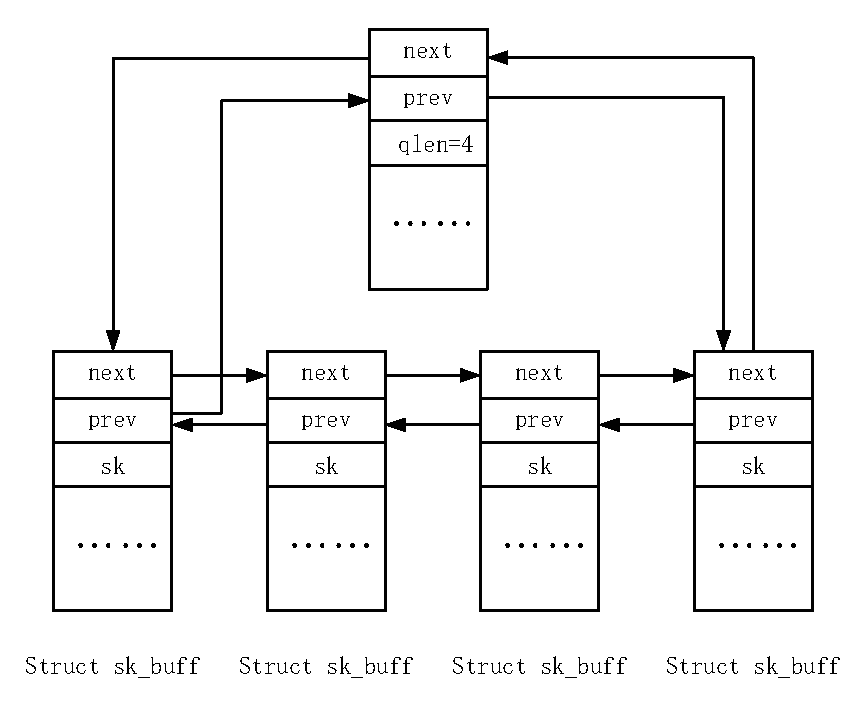
\includegraphics[width=4in]{figures/skbufflink.eps}
	\caption{sk\_buff双向链表}
	\label{SKBUFFLINK_EPS}
\end{figure}
%%%%%%%%%%%%%%%%%%%%%%
\par
编码过程比较简单,算法\ref{algo3}展示了如何对处于编码缓存中的数据包进行编码。当选择的数域足够大时,产生线性相关的编码包的概率可以忽略\textsuperscript{\cite{fragouli2006network}},本文选择在$GF\left(2^8\right)$上进行各种代数运算。
\renewcommand{\algorithmcfname}{算法}
\begin{algorithm}
	\caption{对数据包进行编码} 
	
	\label{algo3}
	\SetKwInOut{Input}{\textbf{输入}}\SetKwInOut{Output}{\textbf{输出}}
	\Input{\\
		冗余度因子 $R$;\\
		编码缓存双向链表 $sk\_buff\_head$;\\
		冗余度残留系数 $NUM$;\\
		编码窗口 $TCPNC\_CODE\_WND$;
	}
	\Output{\\
		编码报文链表 $sk\_buff\_ret$
	}
	$NUM \leftarrow NUM+R$;\\
	\While{$NUM \ge 1$}  
	{  
		从$sk\_buff\_head$表头开始往后遍历$TCPNC\_CODE\_WND$个报文;\\
		在$GF\left(2^8\right)$上生成$TCPNC\_CODE\_WND$个系数;\\
		根据系数和原始数据包计算出编码包;\\
		给编码报文添加NC头部;\\
		将编码包加入到$sk\_buff\_ret$链表;\\
		$NUM \leftarrow NUM-1$;
	}
	\Return \ $sk\_buff\_ret$;
\end{algorithm}
%%%%%%%%%%%%%%%%%%%%%%%%%%%






\subsection{NC层解码缓存}
NC层的解码缓存比较复杂,涉及到数据包解码矩阵;涉及到系数解码矩阵;涉及到3个队列,分别是backlog队列,decoding队列和decoded队列。
\subsubsection{\textbf{解码矩阵}}
解码矩阵分为系数解码矩阵和数据包解码矩阵。
NC解码端收到一个编码包,在判断这个编码包是有效包后,会提取其系数,并找到各个系数在系数解码矩阵中的位置。举个例子说明解码端解码流程。为了简单,下面所有运算都是在实数域,工程实践中是在$GF\left(2^8\right)$下进行运算的。假定解码端先收到编码包$c_{1}=p_{1}$( 这个编码包仅由一个原始数据包$p_{1}$组成 ),那么系数解码矩阵$coeffmat=\left[1\right]$,数据包解码矩阵$pktmat=\left[c_1\right]$。我们得出了$p_{1}+q$,其中$q=0$这种形式,可见$p_{1}$是解出状态,数据包解码矩阵可以重新写为$pktmat=\left[p_{1}\right]$;然后解码端又收到编码包$c_{2}=p_{1}+2p_{2}$,提取其系数1和2,找到其在系数解码矩阵中的位置,并将系数放入其中,有:
\begin{eqnarray}\label{eq31}
	coeffmat=\left[ {\begin{array}{*{20}{c}}
	1&0\\
	1&2
	\end{array}} \right]
\end{eqnarray}
将$c_{2}$放入数据包解码矩阵中,有
\begin{equation}\label{eq32}
pktmat = \left[ {\begin{array}{*{20}{c}}
	{{p_1}}\\
	{{c_2}}
	\end{array}} \right]
\end{equation}
为了看到$p_{2}$( see $p_{2}$ ),我们需要构建$p_{2}=p_{2}+q$,其中$q=\sum\limits_{k = 2} {{a_k}{p_k}} $。
构建$2 \times 2$的单位矩阵$leftmat$,然后对$\left[ {leftmat,coeffmat} \right]$行变换,目标是让$coeffmat$变成上三角矩阵。
\begin{eqnarray}\label{eq33}
\left[ {\begin{array}{*{20}{c}}
	1&0&1&0\\
	{{\rm{ - }}\frac{1}{2}}&{\frac{1}{2}}&0&1
	\end{array}} \right]{\rm{ = }}M \cdot \left[ {\begin{array}{*{20}{c}}
	1&0&1&0\\
	0&1&1&2
	\end{array}} \right]
\end{eqnarray}
式\ref{eq32}中的矩阵$M$代表一系列行变换,可以看到经过一系列行变换后,$coeffmat$已经变为单位阵
\begin{equation}\label{eq34}
leftmat = \left[ {\begin{array}{*{20}{c}}
	1&0\\
	{ - \frac{1}{2}}&{\frac{1}{2}} 
	\end{array}} \right]
\end{equation}
此时,我们只需要将$leftmat$与数据包解码矩阵相乘即可得到$p_{2}$的值。即
\begin{equation}\label{eq35}
\left[ {\begin{array}{*{20}{c}}
	{{p_1}}\\
	{{p_2}}
	\end{array}} \right] = \left[ {\begin{array}{*{20}{c}}
	1&0\\
	{ - \frac{1}{2}}&{\frac{1}{2}}
	\end{array}} \right]\left[ {\begin{array}{*{20}{c}}
	{{p_1}}\\
	{{c_2}}
	\end{array}} \right]
\end{equation}
可知$p_{2}=-\frac{1}{2}p_{1}+\frac{1}{2}c_{2}$,$p_{2}$已解码。此时系数解码矩阵
\begin{eqnarray}\label{eq36}
coeffmat=\left[ {\begin{array}{*{20}{c}}
	1&0\\
	0&1
	\end{array}} \right]
\end{eqnarray}
数据包解码矩阵
\begin{equation}\label{eq37}
pktmat = \left[ {\begin{array}{*{20}{c}}
	{{p_1}}\\
	{{p_2}}
	\end{array}} \right]
\end{equation}
进一步假设,由于链路丢包,$c_{3}=p_{1}+2p_{2}+3p_{3}$丢了,接收端只收到$c_{4}=5p_{2}+4p_{3}+p_{4}$,那么此时的系数矩阵
\begin{eqnarray}\label{eq38}
coeffmat=\left[ {\begin{array}{*{20}{c}}
	1&0&0&0\\
	0&1&0&0\\
	0&5&4&1
	\end{array}} \right]
\end{eqnarray}
值得注意的是,编码包$c_{4}$的三个系数是如何放入系数矩阵的。$coeffmat\left[i\right]\left[j\right]$表示原始数据包$p_{j}$在第$i$个编码包中的系数。此处的序号$j$表示解码矩阵中原始数据包按照起始字节序号从小到大排序的第$j$位。序号$i$表示还残留在解码矩阵的编码包中按照序号排序的第$i$位。值得注意的是,对于解码矩阵第$k$个报文$pktmat[k]$,其内容在一次次的解码中是变化的。例如式\ref{eq32}中$pktmat\left[1\right]=c_2$,在解出$p_2$后,在式\ref{eq37}中$pktmat\left[1\right]=p_{2}$了。
\par
进一步地,取$leftmat$为$3 \times 3$的单位阵,我们对$\left[leftmat,coeffmat\right]$进行行变换,目标是让$coeffmat$成为上三角矩阵
\begin{equation}\label{eq39}
\left[ {\begin{array}{*{20}{c}}
	1&0&0&1&0&0&0\\
	0&1&0&0&1&0&0\\
	0&{ - \frac{5}{4}}&{\frac{1}{4}}&0&0&1&{\frac{1}{4}}
	\end{array}} \right] = M \cdot \left[ {\begin{array}{*{20}{c}}
	1&0&0&1&0&0&0\\
	0&1&0&0&1&0&0\\
	0&0&1&0&5&4&1
	\end{array}} \right]
\end{equation}
上式中$M$代表一系列行变换。此时系数解码矩阵和\emph{leftmat}分别为
\begin{equation}\label{eq310}
coeffmat = \left[ {\begin{array}{*{20}{c}}
	1&0&0&0\\
	0&1&0&0\\
	0&0&1&{\frac{1}{4}}
	\end{array}} \right]
\end{equation}
\begin{equation}\label{eq311}
	leftmat = \left[ {\begin{array}{*{20}{c}}
		1&0&0\\
		0&1&0\\
		0&{ - \frac{5}{4}}&{\frac{1}{4}}
		\end{array}} \right]
\end{equation}
将$c_{4}$放入数据包解码矩阵
\begin{equation}\label{eq312}
	pktmat=\left[ {\begin{array}{*{20}{c}}
		{{p_1}}\\
		{{p_2}}\\
		{{c_3}}
		\end{array}} \right]
\end{equation}
由式\ref{eq310},式\ref{eq311},式\ref{eq312}可得
\begin{equation}\label{eq313}
{p_3} +   \frac{{{p_4}}}{4} = leftmat \cdot pktmat = \left[ {\begin{array}{*{20}{c}}
	1&0&0\\
	0&1&0\\
	0&{ - \frac{5}{4}}&{\frac{1}{4}}
	\end{array}} \right] \cdot \left[ {\begin{array}{*{20}{c}}
	{{p_1}}\\
	{{p_2}}\\
	{{c_3}}
	\end{array}} \right]
\end{equation}
根据式\ref{eq313},得出了$p_{3}+q$,其中$q=\sum\limits_{k = 3} {{a_k}{p_k}} $这种形式,因此接收端这边看到了$p_{3}$。此时,系数解码矩阵为式\ref{eq310},数据包解码矩阵
\begin{equation}
pktmat = \left[ {\begin{array}{*{20}{c}}
	{{p_1}}\\
	{{p_2}}\\
	{{p_3} + \frac{{{p_4}}}{4}}
	\end{array}} \right]
\end{equation}
\par
从上面的例子可以看出,解码端采用流水线解码;系数解码矩阵始终保持着上三角的状态;数据包解码矩阵的每一行在解码运算后始终保持着$p_{i}+q$,其中$q=\sum\limits_{k = i} {{a_k}{p_k}} $ 这样的形式。
\subsubsection{\textbf{backlog队列}}
解码端在收到一个编码报文后,一般会先将其放入到backlog队列。但当组成当前编码数据包的原始数据包中最靠前的一个原始数据包的起始字节序号小于处于数据包解码矩阵中最靠前的原始数据包的起始序号时,这个编码包是无用的,会被丢弃,也就不会放入backlog队列中。逻辑上,在解码端,序号比解码矩阵中最靠前的原始数据包的序号还小的数据包是已经被删除了的,因此如果这个新到的编码包包含这个被删除的原始数据包,解码端也无法将其解出来。backlog队列不会管数据包是否按序到来,只要该编码数据包含有有用信息,就将其加入队列
\par
backlog队列的组织形式为链表。链表优先按构成编码包的原始数据包中的最靠后的原始数据包的起始字节号排序;两者一致的再按先来后到排序。与编码端对sk\_buff的处理不同,这里并没有拷贝sk\_buff结构,而仅仅是通过指针的指向功能构建了一个链表,链表节点数据结构如代码\ref{BACKLOG}所示,其组织形式如图\ref{BACKLOG_EPS}所示。
	\begin{lstlisting}[float,caption=backlog链表节点数据结构,label={BACKLOG},language={[ANSI]C}]
	struct backlog{
		struct backlog *next;
		struct sk_buff *skb;
	}
	\end{lstlisting}

\begin{figure}[htbp]
	\centering
	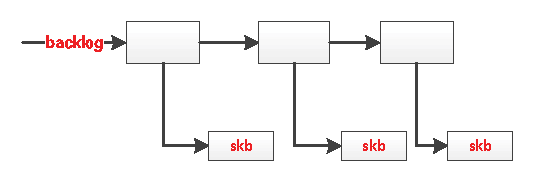
\includegraphics[width=4in]{figures/backlog.eps}
	\caption{backlog链表}
	\label{BACKLOG_EPS}
\end{figure}
\subsubsection{\textbf{decoding队列}}
decoding队列用于存放处在数据包解码矩阵中的数据包,其中有些可能已经被解码,有些还未被解出。其组织形式类似图\ref{BACKLOG_EPS},见图\ref{DECODED_EPS}。decoding队列节点数据结构定义如代码\ref{DECODING}。其中,coeff[TCPNC\_COEFF\_LEN]用于存放处于decoding队列的报文在系数解码矩阵$coeffmat$中的系数;state则表示此报文的状态,decoded状态或者decoding状态。需要注意的是,decoding队列的报文可能已解出,也可能还处于undecoded状态。decoding队列的插入是在遍历backlog队列的过程中发生的,是否可以将某个报文从backlog队列中移到decoding队列需要根据当前的系数解码矩阵\emph{coeffmat}来决定。
\par
如果组成编码包的所有原始数据包的起始序号没有一个是紧接在目前已看到的序号最靠后的原始数据包的后面,那么这个编码包就不应该加入到decoding队列中去。假如目前系数解码矩阵为式\ref{eq310},接收端在收到$c_4$后,又收到$c_5=ap_{5}+bp_{6}+cp_{7}$,如果我们将$c_5$加入decoding队列,同时将相应系数写到系数解码矩阵中,那么系数解码矩阵如图\ref{IFADD_EPS}所示,可以看到$c_5$的加入并不能让我们看到$p_{4}$,因此将其加入decoding队列是无益的。
	\begin{lstlisting}[float,caption=decoding链表节点数据结构,label={DECODING},language={[ANSI]C}]
	struct decoding
	{
	struct decoding *next;
	struct sk_buff *skb;		
	uint8_t coeff[TCPNC_COEFF_LEN];
	unsigned int state;
	};
	\end{lstlisting}
\begin{figure}[htbp]
	\centering
	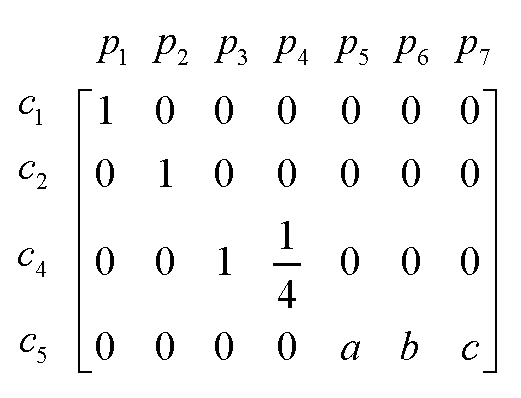
\includegraphics[width=3in]{figures/ifadd.eps}
	\caption{系数解码矩阵示例}
	\label{IFADD_EPS}
\end{figure}
出现这种情况主要由于TCP连接中可能会出现乱序包,或者说由于一连串的丢包,导致新来的当前编码包虽然携带有用信息,但是还不能加入到decoding队列。decoding队列中存在的已解码的原数据包的个数不超过\emph{TCPNC\_CODE\_WND}个。我们不会直接删除decoding队列已解出的报文,而是会将其移出decoding队列,让其离开decoding队列和decoded队列的重合区域,待下次从TCP上层下来的ACK报文到来时,根据其确认序号再对decoded队列中的报文进行删除。
\subsubsection{\textbf{decoded队列}}
decoded队列主要用于存放已经解码出的报文。值得注意的是,decoded队列与decoding队列会有重叠,换句话说,有些数据包既在decoded队列,也在decoding队列,如图\ref{DECODED_EPS}。这是由于已经解码的数据包对于后续的解码可能还有用,因此得以留在解码队列里面。decoded队列与decoding队列的交集不会超过TCPNC\_CODE\_WND个报文。在解码出数据包后,通过调用内核函数ip\_local\_deliver\_finish()\footnote{ip\_local\_deliver\_finish()函数说明参见\url{http://www.embeddedlinux.org.cn/linux_net/0596002556/understandlni-CHP-24-SECT-3.html}}函数将其交给TCP上层。
\begin{figure}[htbp]
	\centering
	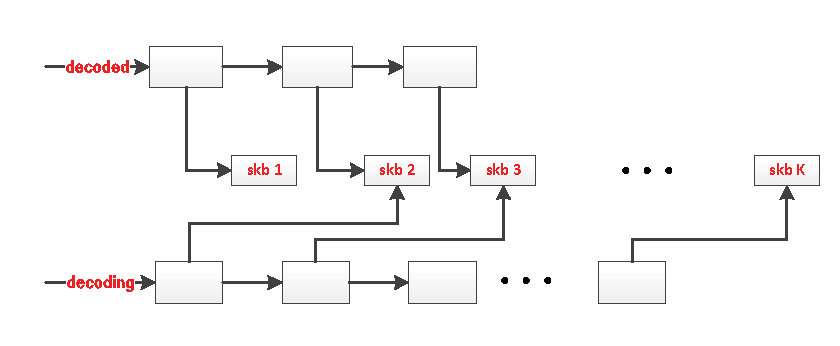
\includegraphics[width=5in]{figures/decoded.eps}
	\caption{decoding队列和decoded队列}
	\label{DECODED_EPS}
\end{figure}
当TCP上层的ACK来到NC层时,可以获知TCP层已确认的字节,然后据此删除decoded队列的数据报文。代码\ref{DECODED}为decoded链表节点数据结构。其中\emph{seqno}表示解码出的数据报文的长度,\emph{length}表示该报文的起始序号,\emph{state}表示该解码包的状态。
	\begin{lstlisting}[float,caption=decoded链表节点数据结构,label={DECODED},language={[ANSI]C}]
	struct decoded
	{
		struct decoded *next;
		struct sk_buff *skb;
		unsigned int seqno;
		unsigned short length;
		unsigned int state;
	};
	\end{lstlisting}
\subsection{接收窗口}
标准TCP中,接收端通过TCP报头的接收窗口值来告诉发送端我这边的接收缓存有多大,好让发送端及时调整发送速度,不至于因为接收端处理不过来导致丢包。考虑到我们在TCP层和IP层插入了一个NC层,而NC层又按照“seen packet”的概念代上层TCP向发送端确认了一些看到了但并没有解出的报文,而这部分报文的字节数是需要从TCP层下来的接收窗口值中减去的。
\par
图\ref{RCVWND_EPS}展示的是如何设置NC层的接收窗口值。$seq_{1}$由NC报头的Base值更新,表示的是发送端那边TCP层中还未被确认的数据中第一个字节的序号;$seq_{2}$由从本地上层TCP下来的报文头部的ACK序号更新,表示NC层已经安全交付给上层TCP的最靠后字节的下一字节序号;$seq_{3}$表示的是NC层提前发给发送端的确认序号,这个序号由看到的报文决定,因此一般会比TCP层的确认序号$seq_{2}$大一些。标准TCP协议中的接收窗口值是根据$seq_{2}$调整的,而NC层积压了一些数据,因此应该根据$seq_{3}$调整接收窗口值。假设从TCP层下来的接收窗口值为$RecvTCP$,NC层在填写NC报头的$RecvWnd$域时,其值应该为$RecvWnd=RecvTCP-\left(seq_{3}-seq_{2}\right)$。
\begin{figure}[htbp]
	\centering
	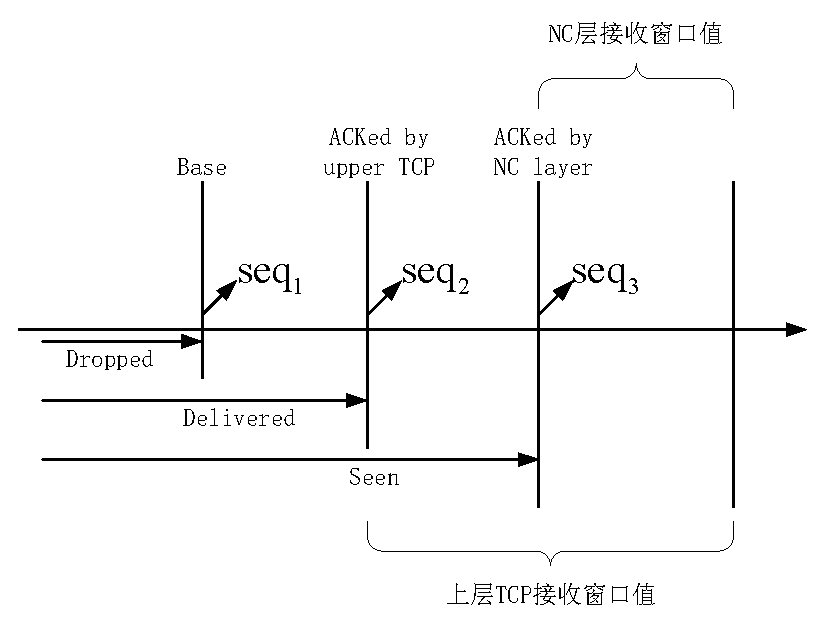
\includegraphics[width=5in]{figures/rcvwnd.eps}
	\caption{接收端NC层窗口值设定}
	\label{RCVWND_EPS}
\end{figure}
\section{测试结果}
本文在Raspberry pi上实现部署了TCP/NC协议,为了精确控制链路的丢包率,我们在接收端的IF\_IP\_PRE\_ROUTING和IF\_IP\_POST\_ROUTING这两处挂载了丢包函数,以概率$\rho$将报文丢弃掉。测试拓扑如图\ref{TUOPU_EPS}。

\begin{figure}[htbp]
	\centering
	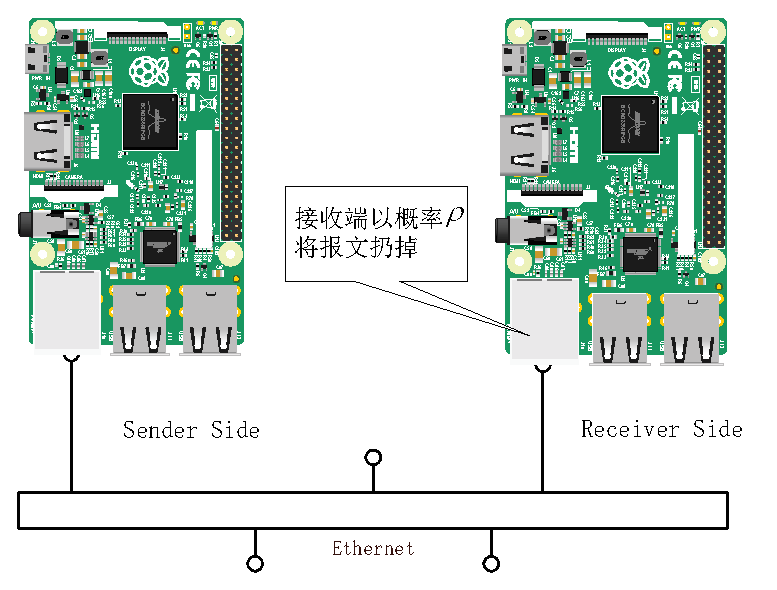
\includegraphics[width=5in]{figures/tuopu.eps}
	\caption{测试拓扑}
	\label{TUOPU_EPS}
\end{figure}
测试环境参数如表\ref{tab:CESHI}。
\begin{table}[htp]
	\centering
	\caption{测试环境参数}
	\label{tab:CESHI}
	\begin{tabular}{ll}
		\toprule
		参数名称&参数值\tabularnewline
		\midrule
		机型		&Raspberry Pi 2 Model B\tabularnewline
		CPU		&900MHz quad-core ARM Cortex-A7 CPU\tabularnewline
		RAM			&1G\tabularnewline
		以太网卡 	&10M/100M\tabularnewline
		操作系统 &Debian\tabularnewline
		内核版本 &Linux 3.18\tabularnewline
		TCP协议版本 &TCP-vegas\tabularnewline
		测试软件 &iperf\tabularnewline
		\bottomrule
	\end{tabular}
\end{table}
设置丢包率$\rho=5\%$,冗余度
\section{本章小结}
